%% LyX 2.1.4 created this file.  For more info, see http://www.lyx.org/.
%% Do not edit unless you really know what you are doing.
\documentclass[a4paper,oneside,brazil,11pt,a4paper,openright,titlepage,usenames,dvipsnames]{book}
\usepackage[utf8]{inputenc}
\usepackage[T1]{fontenc}
\usepackage{lmodern}
\setcounter{secnumdepth}{3}
\setcounter{tocdepth}{3}
\usepackage{array}
\usepackage{verbatim}
\usepackage{listings}
\usepackage{calc}
\usepackage{textcomp}
\usepackage{amssymb}
\usepackage{graphicx}
\usepackage{float}


\lstset{
	aboveskip=6mm,
	belowskip=6mm,
	extendedchars=false,
	escapeinside='',
	showstringspaces=false,
	columns=flexible,
	basicstyle={\small\ttfamily},
	breaklines=true,
	breakatwhitespace=true,
	tabsize=2
}

\renewcommand{\lstlistingname}{Algoritmo}% Listing -> Algorithm
\renewcommand{\lstlistlistingname}{Lista de \lstlistingname s}% List of Listings -> List of Algorithms

\makeatletter

%%%%%%%%%%%%%%%%%%%%%%%%%%%%%% LyX specific LaTeX commands.
\pdfpageheight\paperheight
\pdfpagewidth\paperwidth

%% Because html converters don't know tabularnewline
\providecommand{\tabularnewline}{\\}

%%%%%%%%%%%%%%%%%%%%%%%%%%%%%% User specified LaTeX commands.
% Classe alternativa, apropriada para impressão frente-verso. Inclui páginas em branco
% de forma que capítulos sempre tenham início na página à direita:
% \documentclass[11pt,a4paper,openright,titlepage]{book}

% Pacotes
\usepackage[T1]{fontenc}
\usepackage[brazilian]{babel}
\usepackage{epsfig}
\usepackage{subfig}
\usepackage{amsfonts}
\usepackage{amsmath}
\usepackage[thmmarks,amsmath]{ntheorem}%\usepackage{amsthm}
\usepackage{boxedminipage}
\usepackage{geometry}
\usepackage{theorem}
\usepackage{fancybox}
\usepackage{fancyhdr}
\usepackage{ifthen}
\usepackage{url}
\usepackage{afterpage}
\usepackage{color}
\usepackage{colortbl}
\usepackage{rotating}
\usepackage{makeidx}
\usepackage{indentfirst}
% Pacotes para adição de figuras do inkscape
\usepackage{graphicx}
\usepackage{import}

% Escolher um dos seguintes formatos:
\usepackage{ft2unb} % segue padrão de fontes do Latex

\makeindex

\makeatother

\usepackage{babel}
\begin{document}
\setcounter{secnumdepth}{3}
\setcounter{tocdepth}{2}
\pagestyle{empty}

\grau{Engenheiro de Controle e Automação}

\tipodemonografia{TRABALHO DE GRADUAÇÃO}

\begin{comment}
Título
\end{comment}


\titulolinhai{INTELIGÊNCIA COMPUTACIONAL}
% TODO: validar esse título
\titulolinhaii{PARA AGENTE ÚNICO DE FUTEBOL DE ROBÔS}

\titulolinhaiii{}

\titulolinhaiv{}

\begin{comment}
Autores. Basta retirar o texto totalmente caso não haja um determinado
autor.
\end{comment}


\autori{Bruno Andreghetti Dantas}

\autorii{Samuel Venzi Lima Monteiro de Oliveira}

\autoriii{}

\begin{comment}
Membros da banca. Basta retirar o texto totalmente caso não haja um
determinado membro da banca.
\end{comment}


\membrodabancai{}

\membrodabancaifuncao{}

\membrodabancaii{}

\membrodabancaiifuncao{o}

\membrodabancaiii{}

\membrodabancaiiifuncao{}

\membrodabancaiv{}

\membrodabancaivfuncao{}

\membrodabancav{}

\membrodabancavfuncao{}

\begin{comment}
Data de defesa: mês e ano
\end{comment}

\mes{Maio}
\ano{2021}

\begin{comment}
Comandos para criar a capa e a página de assinaturas
\end{comment}


\capaprincipal
\capaassinaturas

\begin{comment}
Ficha Catalográfica
\end{comment}




\begin{comment}
Dedicatória
\end{comment}


% \frontmatter

\begin{comment}
Texto de dedicatória do primeiro autor.
\end{comment}


% \dedicatoriaautori{um beijo pra minha mãe, pro meu pai, e pra você}

\begin{comment}
Texto de dedicatória do segundo autor. Caso não tenha um segundo autor,
este texto não será mostrado
\end{comment}


% \dedicatoriaautorii{Dedicatória do autor 2}

\begin{comment}
Texto de dedicatória do terceiro autor. Caso não tenha um terceiro
autor, este texto não será mostrado
\end{comment}


% \dedicatoriaautoriii{Dedicatória do autor 3}

\begin{comment}
Comando para criar a página de dedicatória
\end{comment}


% \dedicatoria

\begin{comment}
Agradecimentos
\end{comment}


\begin{comment}
Texto de agradecimentos do primeiro autor.
\end{comment}


\agradecimentosautori{Agradecimentos!}

\begin{comment}
Texto de agradecimentos do segundo autor. Caso não tenha um segundo
autor, este texto não será mostrado.
\end{comment}


\agradecimentosautorii{A inclusão desta seção de agradecimentos é
opcional e fica à critério do(s) autor(es), que caso deseje(em) inclui-la
deverá(ão) utilizar este espaço, seguindo esta formatação.}

\begin{comment}
Texto de agradecimentos do terceiro autor. Caso não tenha um terceiro
autor, este texto não será mostrado.
\end{comment}


\agradecimentosautoriii{A inclusão desta seção de agradecimentos
é opcional e fica à critério do(s) autor(es), que caso deseje(em)
inclui-la deverá(ão) utilizar este espaço, seguindo esta formatação.}

\begin{comment}
Comando para criar a página de agradecimentos
\end{comment}


\agradecimentos

\resumo{resumo}{Resumo!
% TODO: resumo

\medskip{}

Palavras Chave: bla, ble, bli

}\vspace*{2cm}


\resumo{Abstract}{Abstract, in English ofc!
% TODO: abstract

\medskip{}

Keywords: bla, ble, bli

}

\begin{comment}
Listas de conteúdo, figuras e tabelas
\end{comment}


\sumario
\listadefiguras
\listadetabelas


\begin{comment}
Lista de Símbolos
\end{comment}


%TCIDATA{LaTeXparent=0,0,these.tex}


%\chapter*{\setfontarial\mdseries LISTA DE SÍMBOLOS} % se usar ft1unb.sty, descomente esta linha



\chapter*{LISTA DE SÍMBOLOS}

% se usar ft2unb.sty, descomente esta linha


\subsection*{Símbolos}

\begin{tabular}{p{0.1\textwidth}p{0.63\textwidth}>{\PreserveBacklash\raggedleft}p{0.15\textwidth}}
$\pi$ & Política de tomada de ação \tabularnewline
$\gamma$ & Fator de desconto \tabularnewline
$\alpha$ & Fator de aprendizagem \tabularnewline
$\epsilon$ & Fator de exploração \tabularnewline
\end{tabular}

\subsection*{Subscritos}

\begin{tabular}{p{0.1\textwidth}p{0.8\textwidth}}
$*$  & Política ótima \tabularnewline
$t$  & Ciclo $t$ de treinamento \tabularnewline
$terminal$  & Ciclo que encerra episódio \tabularnewline
$q_\pi$ & Função de esperança do retorno de acordo com a política $\pi$ \tabularnewline
\end{tabular}


\subsection*{Siglas}

\begin{tabular}{p{0.1\textwidth}p{0.8\textwidth}}
IA  & Inteligência artificial\tabularnewline
RL & Aprendizagem por reforço - \textit{Reinforcement learning} \tabularnewline
RCSS & \textit{RoboCup Soccer Simulation 2D}\tabularnewline
MDP & Processo de decisão de Markov - \textit{Markov decision process}\tabularnewline
\end{tabular}


\begin{comment}
Corpo Principal
\end{comment}


\mainmatter
\setcounter{page}{1}
\pagenumbering{arabic}
\pagestyle{plain}

\begin{comment}
Introdução
\end{comment}
\chapter{Introdução}
\label{chap:Intro}

% Resumo opcional. Comentar se não usar.
% \resumodocapitulo{Resumo opcional}

\par O interesse humano em criar artefatos para facilitar seu próprio trabalho ou realizar uma tarefa sem interferência remonta os tempos mais antigos. No Egito Ptolomaico, Ctesíbio (285-222 AC) descreveu um relógio d`água com a presença de um sistema de engrenagens, um indicador e o primeiro sistema de retroalimentação registrado. Por volta de 1495, Leonardo da Vinci, concebeu o projeto de um autômato mecânico de um guerreiro em armadura medieval que podia ficar em pé, sentar-se, levantar o visor e mover os braços. \cite{guarnieri2010} 
\par O estudo da união de sistemas eletromecânicos e inteligência teve começo há pelo menos 70 anos. A \textit{cibernética}, área inaugurada por Norbert Wiener na década de 1950, descreve o estudo científico de controle e comunicação no animal e na máquina. Wiener começou, então, a desenvolver sistemas que replicassem comportamentos animais.\cite{wiener1950} Somado a isso, a teoria da informação de Claude Shannon e a teoria de computação de Alan Turing abriram espaço para pesquisas que iriam desenvolver Inteligências Artificiais (IA). \cite{pamela2004} 

\section{Robótica}
\par A robótica se apoia em conhecimentos de vários campos para criar uma das áreas de estudos mais amplas da ciência. Desde a metade do século XX, a robótica vêm reunindo noções dessas áreas, e pouco a pouco as tornando partes essenciais de si: sistemas mecânicos, eletromecânicos, teoria de controle, IA e outras. As aplicações existentes são inúmeras e se renovam a todo momento. Dentre as principais, é possível citar sistemas de manufatura, robótica médica e robótica agricultural. \cite{handbook2007} 
\par Sistemas robóticos construídos para automatizar tarefas repetitivas são interessantes. Entretanto, o avanço das indústrias e aumento da complexidade das tarefas a serem realizadas criou um ambiente catalisador para o desenvolvimento de processos de tomada de decisão autonomamente. 
\par É importante notar a complexidade do problema de se desenvolver a tomada de decisão de um sistema autônomo. Tal sistema precisa mapear seu ambiente por meio de sensores, extrair um significado do seu estado atual, usá-lo para decidir uma ação e determinar se tal ação foi a melhor a ser tomada. Sensores, porém, são imprecisos e limitados fisicamente. A representação dos estados, frequentemente, não é completamente conhecida. E o processo de mapeamento de estado para ação não é trivial.
\par Neste contexto surgiu a área de estudo conhecida como \textit{aprendizagem por reforço}, que formaliza os elementos citados anteriormente para prover uma base de como agentes devem tomar ações para cumprir um objetivo pré-definido. \cite{sutton2018reinforcement}


\section{Aprendizagem por Reforço}
\par A aprendizagem por reforço (do inglês, \textit{reinforcement learning} ou RL) tem como inspiração a maneira como o aprendizado acontece com seres-humanos: interagindo com o ambiente. \cite{sutton2018reinforcement} Se uma criança está aprendendo a andar, por exemplo, ela toma certas ações no ambiente e, ainda que inconscientemente, está atenta aos resultados que essa ação causa. 
\par A teoria por trás da aprendizagem por reforço formaliza a ideia de aprender através da interação e a aplica em um contexto computacional. Os principais elementos de um sistema de RL são: uma política de decisão, um sinal de recompensa e uma função valor.  O primeiro diz respeito à decisão de qual ação se tomar a partir de uma situação, o segundo quantifica quão boa foi a ação escolhida naquele momento e o terceiro quantifica quão boa é a ação considerando o longo prazo.\cite{sutton2018reinforcement}
\par Apesar de recente, a técnica de RL já se mostrou promissora em diversas áreas, com destaque para seu uso em jogos. Em 2016, o programa AlphaGo mostrou resultados significativos ao jogar contra o campeão europeu de Go, superando-o nos 5 jogos que foram disputados. \cite{SilverHuangEtAl16nature}

Em 2018, pesquisadores do grupo OpenAI utilizaram técnicas de RL para treinar um time de 5 agentes colaborativos no jogo \textit{DotA 2}, um jogo de estratégia em tempo real onde 2 times batalham para destruir a base inimiga. O jogo provê um ambiente extremamente complexo, com espaços de estados e ações contínuos. São 20000 números ponto-flutuante para estados e $1.000$ ações possíveis em um dado ciclo.
% Em contrapartida os estados em um jogo de Go são codificados com 400 números e as ações com aproximadamente 250 números.
% retirei essa parte porque achei que tornou confuso se a informação seguinte era sobre Go ou DotA 2
A duração usual de uma partida é de pelo menos 1 hora. Inicialmente, foi feito um sistema do tipo um contra um (1v1) e o agente resultante deste treinamento foi capaz de derrotar jogadores profissionais. Em 2019, o sistema com 5 agentes foi capaz de derrotar um time profissional. \cite{OpenAI_dota} Um resultado dessa magnitude foi possível devido, entre outras razões, ao número altísssimo de amostras coletadas pelos agentes: 300 anos de experiência por dia para o agente singular e 180 anos por dia por agente para o time contendo 5 membros.

\section{Futebol de Robôs}
\par A ideia de robôs jogando futebol foi proposta pela primeira vez em 1992 por Alan Mackworth\cite{mackworth1993seeing}. Desde então a comunidade científica tem criado iniciativas buscando por soluções que tornem isso realidade. Desde então a comunidade científica tem criado iniciativas buscando por soluções que tornem isso realidade.
\par Uma delas é a \textit{Robot World Cup Initiative}, abreviada como \textit{RoboCup}, que teve sua primeira edição em 1997 com mais de 40 equipes distribuídas entre as diversas categorias do evento.
\par O objetivo da iniciativa, definido pela \textit{RoboCup Federation}, é que por volta da metade do século XXI, um time de robôs humanóides autônomos vençam uma partida contra os campeões da Copa do Mundo mais recente. Mesmo que o objetivo pareça ambicioso, ele guia as pesquisas e motiva o avanço no campo.
\par Atualmente, a RoboCup conta com mais de 10 categorias, incluindo robôs humanoides, robôs com rodas e simulações. Entre elas há a \textit{RoboCup Soccer Simulation 2D}, abreviada RCSS, objeto de estudo deste projeto.

\subsection{RoboCup Soccer Simulation 2D}
\par A RCSS possui grande relevância internacional, sendo uma das principais categorias disputadas na RoboCup, com equipes do mundo inteiro.
\par A categoria apresenta, também, grande relevância no cenário brasileiro.
Desde 2005, a RCSS está presente na maior competição de robótica da América Latina, a \textit{Latin American Robotics Competition}, LARC.
\par Nessa categoria, duas equipes de 11 jogadores autônomos e independentes jogam futebol em um ambiente virtual bidimensional. Um servidor é responsável por esse ambiente e possui informação absoluta sobre o estado do jogo e suas regras. Os jogadores, por sua vez, recebem dele informação incompleta e ruidosa de seus sensores virtuais, podendo executar comandos a fim de atuar sobre o estado do jogo. \cite{rcssmanual2003}

\subsection{Servidor da partida}
\label{subsec:server}
\par Um servidor que executa a partida é disponibilizado pelos organizadores da competição e este pode ser utilizado, também, para desenvolvimento. O servidor, portanto, apresenta, internamente, algumas das regras da partida bem como um juiz autônomo que age para determinar gols, faltas e demais situações de uma partida de futebol. Caso necessário, um juiz humano poderá intervir em situações não contempladas pelas regras do servidor.
\par O servidor simula todos os movimentos e ações dos jogadores e da bola. Clientes externos se conectam ao servidor e cada cliente controla um único jogador. A comunição entre o cliente e o servidor é feita a partir do protocolo UDP por meio de mensagens com sintaxe específica e definida pelo servidor.
\par De forma a permitir o acompanhamento visual da partida, um monitor também é disponibilizado, porém não é necessário para que uma partida ocorra com sucesso.
\par O servidor, ainda, possui o modo \textit{trainer} para utilização durante treinamentos de algoritmos de inteligência computacional. Este modo permite a conexão de um cliente do tipo treinador que tem acesso absoluto às informações da partida e pode mudar modos de jogo e ainda mover arbitrariamente jogadores e bola. Adicionalmente, é possível acelerar os ciclos da partida permitindo o treinamento em tempo hábil.

\begin{figure}[h]
	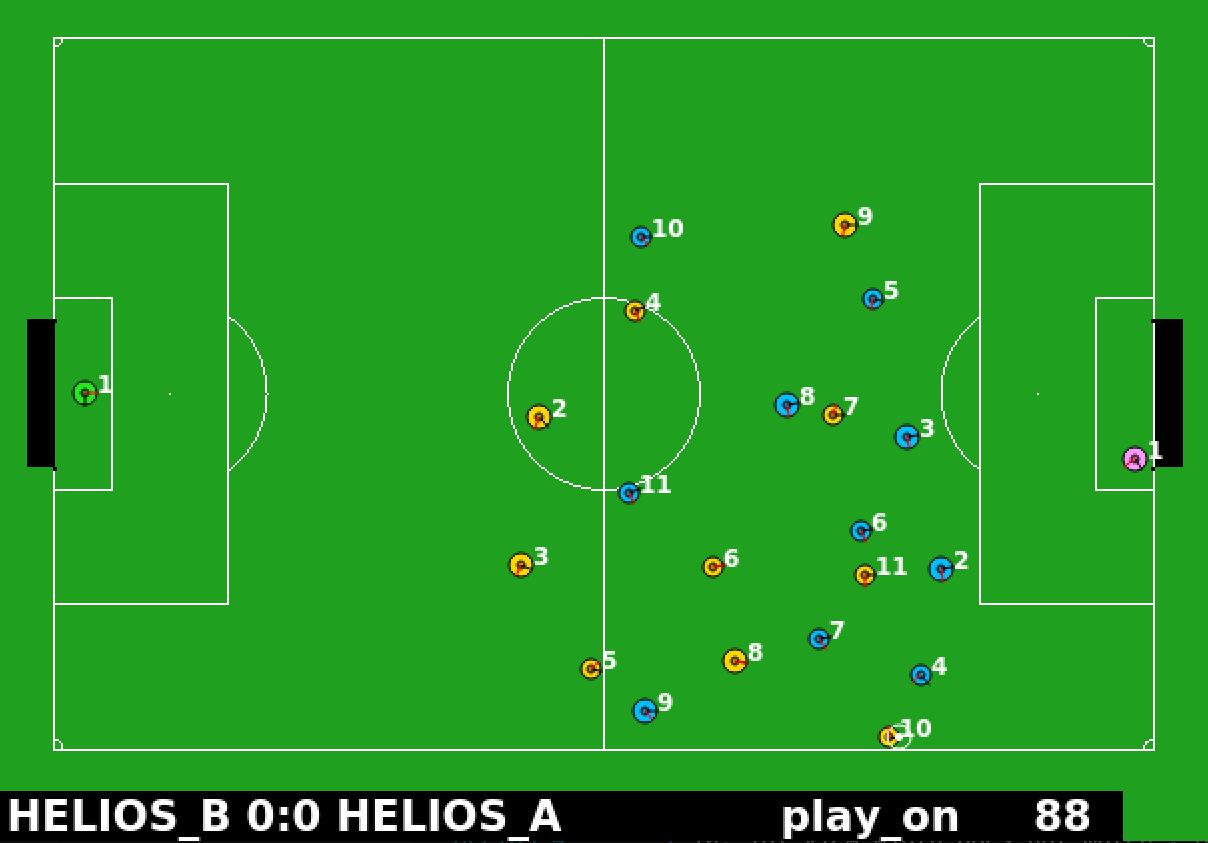
\includegraphics[width=0.7\linewidth]{figs/server.png}
	\centering
	\caption{Visualização de uma partida em andamento}
	\label{fig:rcssserver}
\end{figure}

\subsection{Cliente}
\par Os jogadores são controlados por clientes externos conectados ao servidor. Como já foi dito, um cliente corresponde a um único jogador e os clientes só podem ser comunicar com mensagens mandadas através do servidor da partida.
\par O cliente pode ser desenvolvido em qualquer linguagem desde que se comunique com o servidor pelo protocolo UDP e utilize a sintaxe de mensagens reconhecida pelo sistema. Há várias escolhas disponíveis para a construção do cliente, sendo decisão de cada equipe competidora como fazê-lo.

\begin{figure}[H]
	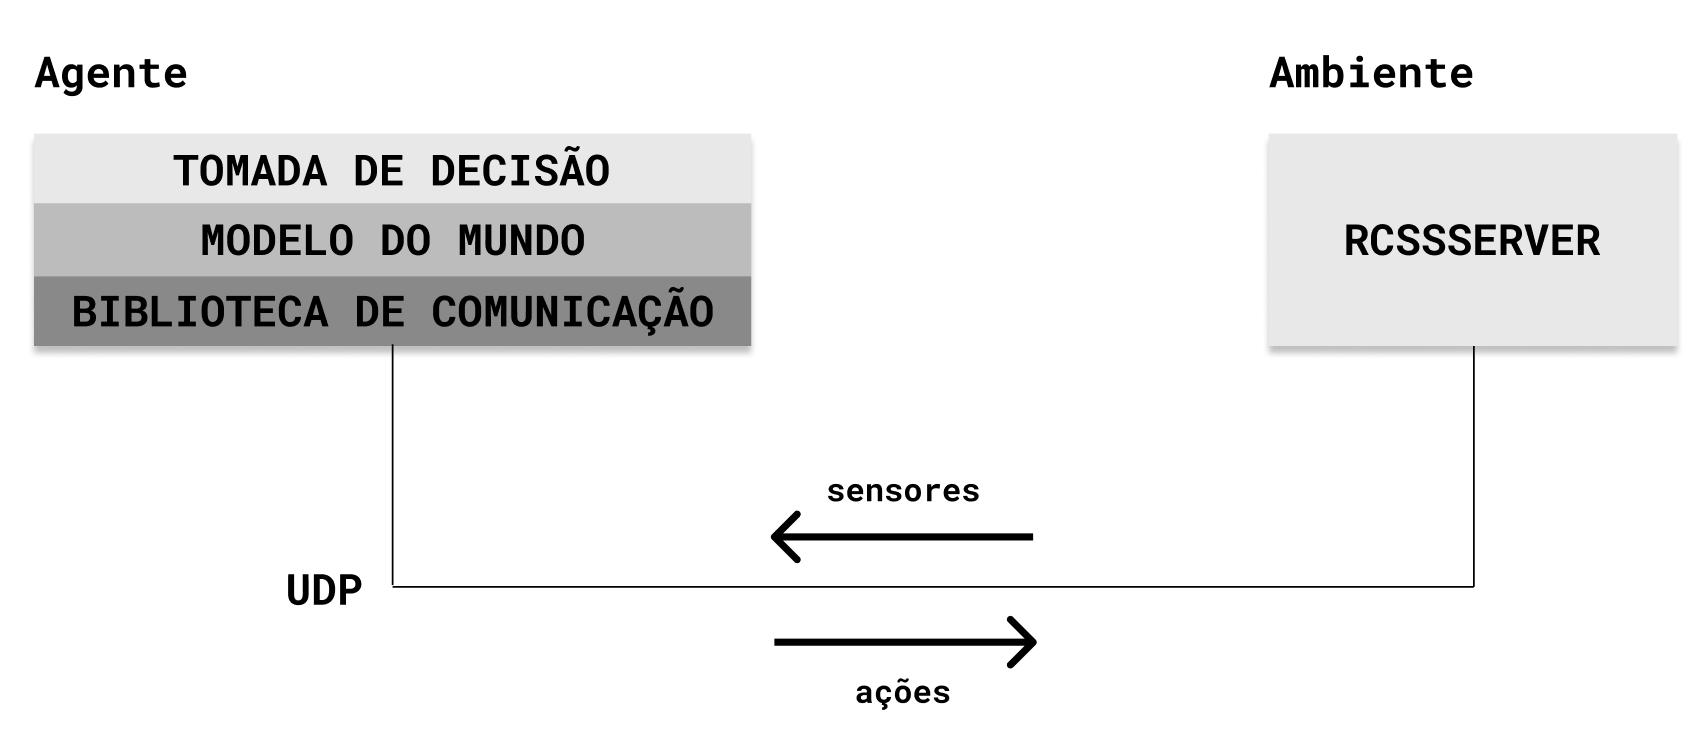
\includegraphics[width=0.9\linewidth]{figs/system.png}
	\centering
	\caption{Esquema ilustrando a arquitetura de um cliente e sua comunicação com o servidor do jogo.}
	\label{fig:system}
\end{figure}

\subsection{Sensores}
\par Cada jogador presente na partida possui um conjunto de sensores de onde são tiradas todas as informações sobre o ambiente. Em uma partida usual, um jogador tem informações visuais dos jogadores do seu time e do time adversário, da bola e de uma série de marcadores fixos no campo, como bandeiras e linhas, que servem para situar o jogador em coordenadas absolutas do campo. O jogador possui também informações ``sonoras'', onde pode ouvir mensagem do árbitro, treinador e de outros jogadores. Por último, tem acesso a informações do próprio corpo, como orientação do corpo e pescoço. \cite{rcssmanual2003}
\par Os sensores possuem características que os aproximam de sensores reais como perda de resolução da informação conforme a variável medida se afasta do sensor.


\subsection{Ações}
\label{sec:actions}

A cada ciclo de simulação, cada cliente conectado ao servidor pode realizar ações que terão efeito no ambiente.\cite{rcssmanual2003}

As ações englobam mover-se, virar-se, chutar a bola e até falar, permitindo troca de mensagens entre os jogadores. As ações disponíveis serão detalhadas no decorrer do texto.


\subsection{Abordagens utilizadas na categoria}
\label{subsec:abordagens}
\par Uma pesquisa sobre as abordagens para o desenvolvimento das estratégias dos times participantes da RCSS revelou o uso recorrente de métodos de inteligência computacional.
\par A equipe chinesa \textit{WrightEagle}, campeã do principal evento internacional da categoria diversas vezes, utiliza Processos de Decisão de Markov ou MDPs para modelar a partida\cite{bai2015online}.
\par A equipe japonesa \textit{HELIOS}, campeã de 2018 da categoria na RoboCup, divide seus jogadores em categorias ``chutadores'' e ``não-chutadores''.
Os chutadores são responsáveis por realizar o planejamento de sequência de ações, utilizando métodos de valor de ação.
Os não-chutadores, por sua vez, não tem conhecimento do planejamento feito pelos chutadores, e devem obter o máximo de informações relevantes para tentar gerar a mesma sequência de ações que jogador chutador\cite{nakashima2018helios2018}.
\par A equipe brasileira \textit{ITAndroids}, atual campeã da LARC, utiliza a abordagem de sequência de ações, similar à \textit{HELIOS}, explorando uma árvore de ações criada dinamicamente de forma a maximizar o valor de cada ação. Além disso, utilizam Otimização por Enxame de Partículas \cite{melloitandroids} para adequar os parâmetros que calculam o valor da ação. A \textit{ITAndroids} também vem desenvolvendo o uso de Aprendizagem por Reforço Profunda \cite{maximoitandroids}.
\par Muitas equipes, ainda, desenvolvem seus agentes utilizando o agente base da equipe \textit{HELIOS}, \textit{Agent2d} com a biblioteca \textit{Librcsc}, escritas em C++. Por isso, é comum que haja semelhança na construção dos agentes dessas equipes.

\section{Caracterização do Problema}
\par Deseja-se, então, explorar o problema de se fazer gols com um agente único no ambiente descrito utilizando-se de técnicas de aprendizagem por reforço.
\par Para isso, foi desenvolvida um biblioteca de interfaceamento com o servidor da partida como adaptação do ambiente. Após isso o agente foi treinado com a utilização de técnicas de RL em duas abordagens - ações puras e comportamentos - de forma a compará-las.
\par No Capítulo 2, descreve-se os fundamentos teóricos da aprendizagem por reforço, com destaque para os algoritmos de \textit{Q-learning} e \textit{Q-learning} duplo. No Capítulo 3, descreve-se o desenvolvimento da biblioteca e a definição de ações e comportamentos. Além disso, propõe-se o algoritmo de treinamento e os experimentos a serem realizados. No Capítulo 4, os resultados desses experimentos e suas análises são apresentados. Finalmente, o Capítulo 5 expõe conclusões e trabalhos futuros.

\subsection{Objetivos}
\par De acordo com o contexto apresentado, o presente trabalho se propõe a cumprir as sequintes etapas:
\begin{itemize}
	\item Implementar uma biblioteca de interfaceamento para comunicação com o servidor
	\item Utilizar técnicas de aprendizagem por reforço para treinar a escolha de ações puras
	\item Utilizar técnicas de aprendizagem por reforço para treinar a escolha de comportamentos
	\item Comparar as diferentes configurações de treinamento e seus resultados
\end{itemize}



\begin{comment}
Fundamentos
\end{comment}
\chapter{Fundamentação Teórica}
\label{chap:Fundamentacao}

% Resumo opcional. Comentar se não usar.
% \resumodocapitulo{Resumo opcional.}


\section{Processos de Decisão de Markov}

O problema abordado neste trabalho pode ser descrito simplificadamente como um Processo de Decisão de Markov (MDP).
MDP é uma forma clássica de representação matemática de processos de decisão sequenciais.
Nesse modelo de representação, cada ação realizada por um agente que interage com o ambiente transforma o estado do processo e determina a recompensa que o agente recebe.
Em um MDP, a codificação do estado atual deve conter toda a informação sobre a interação entre o agente e o ambiente que seja relevante para a dinâmica futura do processo. Nesse caso, é dito que o estado possui a "propriedade de Markov".

\begin{figure}[h]
	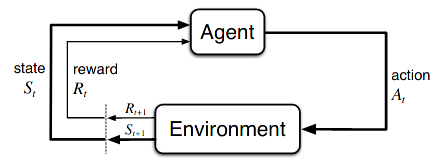
\includegraphics[width=0.6\linewidth]{figs/RL.png}
	\centering
	\caption{Interação agente-ambiente em um MDP \cite{sutton2018reinforcement}.} % figure 3.1 page 48
	\label{fig:mdp_env}
\end{figure}

Assim, dado um espaço de estados $\mathcal{S}$, um espaço de ações $\mathcal{A}$ e um espaço de recompensas $\mathcal{R}$, para cada par $(S, A)$ com $S \in \mathcal{S}$ sendo o estado atual do processo e $A \in \mathcal{A}$ a ação tomada pelo agente, existe uma determinada probabilidade de atingir o estado $S' \in \mathcal{S}$ e receber a recompensa $R \in \mathcal{R}$ \cite{sutton2018reinforcement}.

Essa abordagem é bastante flexível e torna possível modelar a dinâmica do futebol virtual de robôs de diversas maneiras de modo que cada agente possa construir um estado percebido a partir de seus sensores e tomar decisões acerca de qual a melhor ação a fim de maximizar a recompensa recebida.

\subsection{MDP Episódico e Contínuo}

Um MDP pode ser caracterizado quanto à presença de um estado terminal. Caso o MDP tenha um ou mais estados que determinem o fim do processo, ele é dito episódico e a totalidade do processo até o estado que determina o fim é chamada de episódio. A simulação de futebol de robôs tratada neste trabalho é um exemplo de MDP episódico, uma vez que o MDP termina ao se encerrar o tempo de jogo.

Em contrapartida, há MDPs nos quais não está bem definido nenhum estado terminal. Nesses casos, o MDP pode continuar indefinidamente até uma ação externa ao MDP determinar a sua parada. Um exemplo disso é um MDP que controle um robô numa linha de produção. Caso o sistema de automação supervisor desse robô não determine sua parada (por falta de insumos, por exemplo), o MDP pode seguir operando indefinidamente.

% Nesta fundamentação, será tratado com mais atenção o caso episódico uma vez que é o caso que interessa para aplicação na simulação de futebol de robôs.
% (comentei fora essa parte porque a gente acabou fazendo o algoritmo contínuo usando o gamma lá porque a gente não codificou o tempo de jogo no estado)

\subsection{Recompensa e Retorno}

Como definido acima, é atribuída uma recompensa $R \in \mathcal{R}$ para cada ação tomada em um MDP. Essa recompensa é sempre referente ao instante de tempo anterior, ou seja, não depende de qualquer outro fator que não o par $(S_t, A_t)$ executado no instante $t$ e a função de probabilidade associada pelo MDP a esse par. Por isso, é comum utilizar a notação $R_{t+1}$ para se referir à recompensa obtida após tomar a ação $A_t$ no instante de tempo $t$.

Porém, em muitos casos, é esperado de um agente que ele tome decisões para maximizar a recompensa total a longo prazo, ou seja, em um MDP episódico é esperado que se escolha $A_t$ a fim de maximizar não apenas $R_{t+1}$ mas sim o retorno $G_{t}$ tal que:

\begin{equation}
G_{t} = R_{t+1} + R_{t+2} + \dotsc + R_{terminal}.
\end{equation}

Caso o MDP seja contínuo, $G_t$ pode divergir, uma vez que é uma soma infinita de parcelas. Para solucionar o problema, basta adicionar à equação um fator de desconto ($\gamma$), tal que seja possível ajustar a relevância de recompensas futuras para o cálculo do retorno:

\begin{equation}
	G_{t} = R_{t+1} + \gamma R_{t+2} + \gamma^2 R_{t+3} + \dotsc = \sum_{k=1}^{\infty} \gamma^k R_{t+k+1}.
\end{equation}
% 
Observa-se que, para $ 0 \leq \gamma < 1$, o somatório converge. Para $\gamma = 0$, o retorno leva em consideração apenas a recompensa imediata $R_{t+1}$. Em contrapartida, para $\gamma \to 1$, as recompensas mais distantes no futuro são cada vez menos descontadas, ou seja, o agente tende a levar mais em consideração os ganhos futuros.

\subsection{Políticas e Funções de Valor}

É dado o nome de política para qualquer função $\pi: (S, A) \to \mathbb{R}$ que associe um estado qualquer do MDP e uma ação a uma probabilidade de se tomar essa ação diante desse estado, ou seja, $\pi(A|S) = p$ onde $p$ é a probabilidade de selecionar a ação A diante do estado S.

Para cada política $\pi$ existe uma função $v_\pi: (S) \to \mathbb{R}$ que, para cada estado, define a esperança de retorno caso o agente continue seguindo a política $\pi$. A função $v_\pi$ é conhecida como função de valor sob a política $\pi$.

Similarmente, existe uma função $q_\pi: (S, A) \to \mathbb{R}$ que, para cada par de estado e ação, define a esperança de retorno. Neste caso, a função $q_\pi$ é conhecida como função de valor da ação sob a política $\pi$.

É possível comparar duas políticas $\pi$ e $\pi'$ a respeito de suas funções $q$. A política $\pi$ é considerada melhor ou igual a $\pi$, ou $\pi \ge \pi'$, caso $q_\pi(S, A) \ge q_{\pi'}(S, A)$ para todo par $(S, A)$.

Sempre há ao menos uma política melhor ou igual a todas as outras, denominada política ótima. Qualquer política que cumpra esse requisito é denominada $\pi_*$ e, caso haja mais de uma, todas devem possuir a mesma função $q$ denominada $q_*$ \cite{sutton2018reinforcement}. No decorrer deste trabalho serão utilizadas técnicas que buscam estimar $q_*$. % chap 3.6 

Uma política que toma sempre o caminho de maior retorno é denominada gulosa e uma política que toma o caminho de maior retorno mas escolhe uma ação aleatoriamente com probabilidade parametrizada $\epsilon$ é denominada $\epsilon$-gulosa.


\section{Aprendizagem por Reforço}

Dada uma modelagem do problema como um MDP, resta obter uma maneira de estimar as probabilidades que descrevem a dinâmica desse MDP para determinar a política capaz de maximizar a recompensa a longo prazo recebida pelo agente. O conjunto de técnicas que resolvem esse tipo de problema é chamado de Aprendizagem por Reforço.

No campo da aprendizagem de máquina, ela se difere da Aprendizagem Supervisionada por não haver um conjunto de pares $(s, a)$ conhecidos a partir de exemplos.
Nesse tipo de aprendizagem, o objetivo é extrapolar uma solução genérica a partir de exemplos de um conjunto de treinamento dado como correto, o que não é prático em problemas em que não se tem exemplos de comportamentos esperados e que representem bem o conjunto total de situações possíveis.
Ela também se diferencia da Aprendizagem Não-Supervisionada, que tradicionalmente visa encontrar estrutura em conjuntos de dados não classificados, enquanto a Aprendizagem por Reforço visa maximizar um sinal de recompensa \cite{sutton2018reinforcement}.

Desse modo, as técnicas de Aprendizagem por Reforço serão aplicadas a fim de buscar políticas capazes de maximizar o desempenho dos jogadores virtuais, ou seja, obter políticas que tornem os agentes capazes de fazer gols e evitar que os jogadores do time adversário façam gols.

\subsection{Aprendizagem com Diferença Temporal}
\par A aprendizagem com diferença temporal (\textit{temporal-difference learning}, ou TD) é uma das ideias centrais de RL \cite{sutton2018reinforcement}. Esse tipo de aprendizado é importante pois permite o aprendizado sem um modelo prévio do MDP do ambiente e também permite o uso de estimativas aprendidas durante o treinamento, conhecido como \textit{bootstrapping}, acelerando dramaticamente o tempo de convergência. 
\par A diferença temporal se apoia na ideia de que a política aproximada e a função de valor devem se relacionar de forma que ambas convirjam para seus valores ótimos, conhecida como iteração generalizada da política (\textit{generalized policy iteration} ou GPI) \cite{sutton2018reinforcement}. 
\par As técnicas \textit{Sarsa}, \textit{Q-learning} e \textit{Double Q-learning} apresentadas nas Subseções \ref{subsec:sarsa-theory}, \ref{subsec:q-theory} e \ref{subsec:dq-theory} são exemplos de aprendizagem com diferença temporal.

\subsection{Aprendizagem On-policy e Off-policy}
\label{subsec:on-off-policy}
Entre as técnicas de aprendizagem por reforço, existe uma divisão entre a aprendizagem on-policy e a aprendizagem off-policy, referentes à relação entre a política executada durante o aprendizado e a política sobre a qual se quer aprender.

Nos algoritmos de aprendizagem on-policy o agente aprende a respeito da política $\pi$ enquanto navega o MDP de acordo com a própria política $\pi$, ou seja, a política executada durante a aprendizagem é a mesma que se quer estudar.

Em contrapartida, nos algoritmos de aprendizagem off-policy o agente aprende a respeito da política alvo $\pi$ enquanto navega o MDP de acordo com a política $b$, ou seja, ele estima a função $q_{\pi}$ enquanto executa a política $b$. Esses métodos costumam introduzir variância no processo, tornando o aprendizado ruidoso e muitas vezes divergente.

Além disso, é possível observar que a aprendizagem on-policy é apenas um caso particular da aprendizagem off-policy em que $b = \pi$.

\subsection{Soluções Tabulares e Aproximadas}

A maioria dos métodos de aprendizagem por reforço são testados e validados em MDPs cujos espaços de estados $\mathcal{S}$ e de ações $\mathcal{A}$ são suficientemente pequenos. Para esses MDPs é possível utilizar uma solução tabular, ou seja, a função $Q$ poda ser armazenada em uma tabela de tamanho razoável e sua imagem para cada par estado-ação pode ser atualizado individualmente.

Infelizmente, em diversas aplicações a quantidade de estados possíveis é grande demais ou até mesmo infinita, como é o caso de sistemas em que determinada característica do estado é medida como uma grandeza contínua. Nesses casos, é impossível esperar que se obtenham soluções ótimas mesmo com tempo infinito, portanto o objetivo é obter uma solução aproximada que seja boa o suficiente para a aplicação desejada.

A ferramenta matemática utilizada para viabilizar soluções aproximadas é o conceito de aproximadores de função, muito utilizados na aprendizagem supervisionada. Entre os aproximadores mais utilizados, estão os aproximadores lineares e as redes neurais multicamada.

\subsection{A Tríade da Morte}

Sutton e Barto definem um cenário denominado a tríade da morte (\textit{the deadly triad}) como um cenário onde a presença de três elementos causa instabilidade e divergência em treinamentos: aproximação de funções, \textit{bootstrapping} e treinamentos off-policy \cite{sutton2018reinforcement}.

Existe, portanto, a decisão do projetista de definir treinamentos de forma a evitar o conjunto desses três elementos. O aproximador de funções pode ser evitado com técnicas tabulares em ambientes menos complexos e ao custo de uso de memória. Para métodos TD, \textit{bootstrapping} é um requerimento. Entretanto, outros métodos permitem realizar o treinamento sem o uso de estimativas. Métodos off-policy são considerados mais poderosos e versáteis, porém introduzem mais variância como descrito na Subseção \ref{subsec:on-off-policy} e, portanto, nem sempre são a melhor escolha.

\subsection{\textit{Exploration} e \textit{Exploitation}}

A realização do treinamento de um agente por RL tem como principal pilar a visita desse agente a estados diferentes e escolha de ações para que seja adquirido conhecimento sobre quais recompensas são maiores para o par $(S,A)$. A exploração desses estados desconhecidos (\textit{exploration}, em inglês) tem sentido de pesquisa ou estudo com o objetivo de obter novas informações sobre o ambiente.

Oposto a isso, após obter-se conhecimento suficiente sobre o ambiente, o treinamento deve mudar seu foco para tirar proveito do que foi aprendido, passando a revisitar os estados e tomar as ações que maximizem a recompensa. Nesse caso, exploração (\textit{exploitation}, em inglês) tem sentido de tirar vantagem ou proveito de uma situação já conhecida.

É necessário, então, balancear os dois tipos de exploração de forma a direcionar o treinamento. Isso pode ser feito, simplesmente, com uma probabilidade de se tomar uma ação aleatória adicionada à política de decisão: o fator de exploração $\epsilon$. Esse fator está no intervalo $[0, 1]$, onde $1$ representa $100\%$ de chance de uma ação aleatória ser escolhida. O fator $\epsilon$ é inicializado arbitrariamente alto, para encorajar a exploração de estados desconhecidos e decai de acordo com alguma parametrização para que o agente passe a tirar proveito de situações já conhecidas.

\subsection{Sarsa}
\label{subsec:sarsa-theory}
Entre os algoritmos de aprendizagem on-policy está o Sarsa. Seu nome é derivado da quíntupla $(S_t, A_t, R_{t+1}, S_{t+1}, A_{t+1})$ utilizada como entrada da sua fórmula de atualização:

\begin{equation}
	\label{eq:sarsa}
	Q(S_t, A_t) \leftarrow Q(S_t, A_t) + \alpha[R_{t+1} + \gamma Q(S_{t+1}, A_{t+1}) - Q(S_t, A_t)].
\end{equation}

Uma vez que a política adotada pelo agente não pode ser gulosa, pois inibiria a exploração do espaço de estados e de ações, é interessante que o agente siga uma política $\epsilon$-gulosa baseada na estimativa de $Q$. Nesse caso, para Q tabular, a convergência para a política ótima é garantida desde que todos os pares $(S, A)$ sejam visitados infinitas vezes e a política convirja para a política gulosa em $t \to \infty$.

Para o caso em que se usa um aproximador para estimar Q não há garantias, porém a natureza on-policy do Sarsa reduz a variância da aprendizagem. Isso pode tornar essa abordagem mais estável do que o Q-learning, descrito a seguir.

\subsection{Q-Learning}
\label{subsec:q-theory}
Um dos algoritmos mais populares no campo da aprendizagem por reforço é o Q-Learning. Trata-se de um método off-policy que aproxima diretamente a função $q_*$ independente da política que estiver sendo adotada pelo agente durante o treinamento.

O algoritmo é também muito simples. Dada uma representação tabular $Q: (\mathcal{S},\mathcal{A}) \to \mathbb{R}$ da função $q_*$, para cada instante de tempo $t$ é realizada a seguinte atualização a fim de aproximar $Q$ de $q_*$:

\begin{equation}
Q(S_t, A_t) \leftarrow Q(S_t, A_t) + \alpha[R_{t+1} + \gamma\max_{a} Q(S_{t+1}, a) - Q(S_t, A_t)],
\end{equation}
% 
sendo $\alpha$ o fator de aprendizagem, responsável por suavizar o impacto de cada atualização da tabela, e $\gamma$ o fator de desconto, responsável por reduzir a relevância de recompensas muito distantes no tempo.

Após iterações suficientes, espera-se que $Q$ convirja para $q_*$. Em certas condições a convergência é matematicamente garantida.

Uma vez estimada a função $q_*$, é simples obter a política ótima. Basta escolher a ação que maximiza $q_*$ no estado atual, ou seja:

\begin{equation}
A_{t} = \max_{a} q_*(S_t, a).
\end{equation}

É comum, mas não obrigatório, que a política $b$ seguida durante o aprendizado seja $epsilon$-gulosa em relação à aproximação $Q$.

\subsection{Q-Learning Duplo}
\label{subsec:dq-theory}
Apesar de popular, o Q-Learning possui um problema de viés de maximização. Uma vez que a aproximação $Q$ é imprecisa no início do treinamento, é possível que o retorno esperado estimado seja enviesado para um valor maior do que o real.

Como solução para esse problema, é utilizada a abordagem do Q-Learning Duplo. Nela são utilizadas duas aproximações, $Q_1$ e $Q_2$, e a atualização de $Q$ é dada da seguinte forma:

\begin{equation}
\label{eq:doubleq}
Q_1(S_t, A_t) \leftarrow Q_1(S_t, A_t) + \alpha[R_{t+1} + Q_2(S_{t+1}, \text{arg}\max_a Q_1(S_{t+1}, a)) - Q_1(S_t, A_t)].
\end{equation}
% 
Em metade das iterações (através de um sorteio, por exemplo), as aproximações $Q_1$ e $Q_2$ são trocadas. Com isso, é anulado o viés de maximização gerado pelo uso de $\max_a Q$ como estimativa de retorno para os estados seguintes.

Outra vantagem desse método é que, apesar de dobrar os requisitos de memória do algoritmo por ser preciso armazenar os dados referentes a duas aproximações, ele não aumenta o custo computacional por iteração.

No capítulo seguinte estão descritos o desenvolvimento da plataforma de testes e também os experimentos realizados para validá-la.

\begin{comment}
Desenvolvimento
\end{comment}
\chapter{Desenvolvimento \label{chap:Desenvolvimento}}

% Resumo opcional. Comentar se não usar.
% \resumodocapitulo{Resumo opcional.}


\section{Biblioteca} \label{sec:lib}

O servidor da partida apresenta, como já mencionado, um protocolo de comunicação e sintaxe de mensagens específica. Uma biblioteca de interfaceamento foi desenvolvida com o objetivo de abstrair os detalhes de comunicação de construção de mensagens e facilitar, assim, o desenvolvimento dos programas jogadores. Esta abordagem já é comum na categoria e existem soluções de código aberto como a \textit{librcsc}, utilizada por várias equipes, usualmente atreladas ao agente base \textit{agent2d}, desenvolvidas pela equipe \textit{HELIOS}.

A biblioteca própria foi desenvolvida em linguagem Go como forma de modernização e diversificação da base de código utilizada pelas equipes. A biblioteca cobre uma parte considerável das possibilidades previstas no protocolo de comunicação e foi programada de modo a ser facilmente expansível de acordo com o lançamento de novas versões do servidor.

% TODO melhorar isso aqui

\subsection{Arquitetura}
A biblioteca possui três pacotes internos: \textit{playerclient}, \textit{trainerclient} e \textit{rcsscommon}. Os dois primeiros dizem respeito aos dois tipos de programas que podem se conectar ao servidor da partida: jogadores e treinadores. O terceiro engloba todas as funcionalidades utilizadas por ambos clientes, além de informações gerais sobre parâmetros da partida, como coordenadas de bandeiras do campo e modos de jogo.

Os dois clientes desenvolvidos possuem as funcionalidades necessárias para se conectar ao servidor, ouvir mensagens via protocolo UDP, decodificá-las e então executar uma ação em forma de mensagem codificada e enviada ao servidor.

\subsection{Decodificação de Codificação de Mensagens}
% ( // tradução de parser)
A decodificação de mensagens, por sua vez, foi feita em duas camadas: um \textit{lexer} e um analisador. O lexer passa pelas mensagens em formato string e retira todas as informações que ela contém. O analisador estrutura essas informações em estruturas de dados para que possam ser utilizadas fora da biblioteca. As informações recebidas e decodificadas são, em sua maioria, dados dos sensores do jogador.
\begin{center}



\begin{tabular}{c}
\begin{lstlisting}
(see 37 ((f c b) 16.6 -1 -0 -0.8))
\end{lstlisting}
\end{tabular}

Exemplo de mensagem codificada.


\begin{tabular}{c}
\begin{lstlisting}
SightSymbols{
	Time: 37,
	ObjMap: map[string][]string{
		"f c b":    {"16.6", "-1", "-0", "-0.8"},
	},
}
\end{lstlisting}
\end{tabular}

Mensagem após passar pelo \textit{lexer}.



\begin{tabular}{c}
\begin{lstlisting}
SightData{
	Time: 37,
	Ball: nil,
	Lines: LineArray{},
	Flags: FlagArray{
		{
			ID:        rcsscommon.FlagCenterBot,
			Distance:  16.6,
			Direction: -1,
		},
	},
}
\end{lstlisting}
\end{tabular}

Mensagem após passar pelo analisador.

\end{center}

\section{Experimentos}

\subsection{Ambiente de Treinamento}

O ambiente de treinamento consiste em uma base de código que importa a biblioteca detalhada na seção \ref{sec:lib}. Um formato geral foi definido e desenvolvido a fim de tornar os experimentos fáceis de adaptar, bastando mudar alguns trechos do código.

Além disso, para os dados disponíveis por meio da biblioteca foram estimados outros estados que pudessem ser úteis no treinamento: posições absolutas da bola, dos outros jogadores e do próprio jogador.

\subsubsection{Laço de Treinamento}

De forma geral o laço de treinamento obedece o pseudo-código apresentado.

\begin{tabular}{c}
	\begin{lstlisting}
definir parametros
inicializar pesos de treinamento
laco para cada partida:
	conectar jogador
	laco para cada passo da partida:
		ver estado
		escolher acao de acordo com uma politica
		observar novo estado e recompensa
		treinar pesos
		estado <- novo estado
		se estado for terminal:
			quebra
	\end{lstlisting}
\end{tabular}

O laço interno é onde efetivamente os algoritmos de treinamento são implementados, portanto este trecho é alterado a depender da técnica de aprendizagem por reforço utilizada.

\subsubsection{Estimação de Estados}

Os sensores do jogador fornecem somente informações em coordenadas polares relativas ao próprio jogador. Desta forma, ele possui informações de distância e direção para a bola, demais jogadores, bandeiras do campo e linhas do campo. 

Com esses dados, entretanto, é possível estimar as coordenadas cartesianas absolutas no campo de todas as entidades de interesse. As bandeiras do campo são fixas e possuem coordenadas conhecidas. Portanto, a transformação da informação polar e relativa para uma cartesiana e absoluta da posição do próprio jogador é direta utilizando trigonometria básica. 

A partir da informação de posição absoluta do próprio jogador e de sua direção é possível calcular as posições para o resto das entidades.


\subsection{Agente Único com Double Q-Learning Tabular}

% Inicialmente, deseja-se realizar o treinamento de um agente único que, com as informações de seus sensores, consiga com sucesso levar a bola ao gol. Essa proposta tem como objetivo fundamentar os conhecimentos e validar a base de código para a realização de um treinamento de um time de múltiplos agentes em um estágio posterior.

% O desenvolvimento de um agente único, inicialmente, permite adquirir o entendimento necessário para a definição do vetor de estados e ajuste das técnicas de treinamento. Além disso, busca-se uma maior agilidade na substituição e teste na estrutura do vetor de estados e no algoritmo de treinamento, uma vez que o custo computacional deste cenário é consideravelmente menor que o custo do treinamento de um time completo.

O objetivo inicial para teste do sistema como um todo foi o de realizar o treinamento de um agente único capaz de executar gols estando sozinho em campo. Esse objetivo se provou mais difícil do que o esperado para a abordagem \textit{end-to-end} desejada.

Foi utilizado o algoritmo Double Q-Learning tabular, possível através da discretização de diversas métricas obtidas através dos sensores do agente.

\subsubsection{Codificação dos Estados}

O estado percebido pelo agente é dado pela combinação dos seguintes fatores:

\begin{itemize}
    \item \textbf{Distância até a bola}. A distância $D$ até a bola foi discretizada de acordo com a seguinte função:
    \begin{equation}
    \label{eq:balldist}
    \left\{
        \begin{array}{ll}
            0  & \mbox{se } D < 0.7 \\
            \lfloor\log_2 (\frac{D}{0.7})\rfloor & \mbox{se } 0.7 \leq D \mbox{ e } D < 0.7 \times 2^6 \\
            6  & \mbox{se } D \geq 0.7 \times 2^6 \\

        \end{array}
    \right.
    \end{equation}

    Ou seja, a distância percebida até a bola varia entre 0 e 6 com resolução cada vez menor à medida que o agente se afasta da bola. O fator 0.7 foi inserido na função devido ao fato de que esta é a distância mínima que permite que o agente chute a bola.

    Caso o jogador possa enxergar a bola, a distância D é recebida diretamente do sensor. Caso contrário, a distância D é estimada com base na última posição percebida da bola.

    \item \textbf{Direção da bola}: A direção da bola foi dividida em 24 fatias de $15^{\circ}$ cada. O ângulo de visão do jogador é de $\pm30^{\circ}$. Caso a bola não esteja visível, a direção da bola é estimada com base na última posição percebida.
    
    \item \textbf{Posição do jogador em X}: A posição estimada do jogador em X foi discretizada em 10 janelas de tamanho $11.5$.

    \item \textbf{Posição do jogador em Y}: A posição estimada do jogador em Y foi discretizada em 7 janelas de tamanho aproximado $11.14$.
    
    \item \textbf{Direção do jogador}: A direção estimada do jogador em relação ao eixo horizontal foi discretizada em 24 fatias de $15^{\circ}$ cada.

\end{itemize}

Com isso, temos que o número total de estados possíveis é dado pelo produtório da quantidade de possibilidades em cada um dos itens acima totalizando 282240 estados.

\subsubsection{Codificação das Ações}

Para simplificar o vasto espaço de ações disponíveis, foi selecionado um conjunto discreto de 13 ações:

\begin{itemize}
    \item \textbf{Ação nula}: O agente apenas espera até o próximo ciclo.

    \item \textbf{Virar-se}: O agente tem a opção de virar-se $7^{\circ}$, $15^{\circ}$ ou $31^{\circ}$ para ambas as direções, totalizando 6 ações de rotação possíveis. 
    
    \item \textbf{Correr}: É possível correr em frente ($0^{\circ}$) ou a $30^{\circ}$ em ambas as direções, sempre com potência 50, totalizando 3 ações de corrida possíveis.

    \item \textbf{Chutar}: Caso a distância até a bola seja menor ou igual a 0.7 metros, o jogador tem a opção de chutá-la em frente ou em um ângulo de $45^{\circ}$ em ambas as direções, totalizando 3 ações de chute possíveis. Caso a bola não esteja próxima o suficiente, nada acontece.
\end{itemize}

\subsubsection{Parâmetros}

\begin{itemize}
    \item \textbf{Fator de desconto ($\gamma$)}: Apesar do ambiente ser episódico, foi utilizado um fator de desconto de 0.99 devido ao fato de que a condição de término do episódio (fim de jogo) não ser observável através da discretização do estado utilizada.  

    \item \textbf{Fator de aprendizagem ($\alpha$)}: O fator de aprendizagem foi definido inicialmente como 0.1 e foi reduzido exponencialmente multiplicando-o por $0.99999$ ao final de cada partida. 
    
    \item \textbf{Fator de exploração ($\epsilon$)}: Para incentivar a exploração das possibilidades, o fator de exploração foi definido inicialmente como 0.9 e reduzido exponencialmente multiplicando-o por $0.99996$ ao final de cada partida. A cada ação tomada, o agente tem probabilidade $\epsilon$ de escolher uma ação aleatória. Além disso, para favorecer a exploração, no início de cada partida era também sorteada uma posição inicial para o agente em seu lado do campo.
\end{itemize}

\subsubsection{Recompensa}

A recompensa foi definida em 3 partes a fim de guiar o agente na direção do aprendizado desejado. Todas as medições de recompensa foram feitas utilizando dados da simulação e não da percepção do agente.

\begin{itemize}
    \item \textbf{Proximidade da bola $R_1$}: Para que o agente tenha tendência a se aproximar da bola, foi definida uma recompensa negativa proporcional à distância $d$ do agente em relação à bola, ou seja: $R_1 = -d*0.001/6000$.

    \item \textbf{Velocidade da bola $R_2$}: Para que o agente adquira o comportamento de chutar a bola em direção ao gol adversário, foi definida uma recompensa positiva proporcional à velocidade instantânea da bola em X ($v_x$), ou seja: $R_2 = v_x/6000$.
    
    \item \textbf{Gol $R_3$}: Por fim, para incentivar que o agente fizesse gols, foi definida uma recompensa esparsa de valor 1 para cada gol realizado e -1 para gols contra, ou seja:
    
    $
    R_3 =
    \left\{
        \begin{array}{ll}
        \ \ 1  & \mbox{se foi feito um gol no ciclo} \\
         -1  & \mbox{se foi feito um gol contra no ciclo} \\
        \ \ 0  & \mbox{caso não houver gol no ciclo} \\
        \end{array}
    \right.
    $
\end{itemize}

Deste modo, a cada instante de tempo foi atribuída uma recompensa $R = R_1 + R_2 + R_3$.

\subsubsection{Procedimentos e Resultados}

Foram executados 2 treinamentos distintos de 100000 partidas a fim de suavizar o elemento sorte nos resultados. Após cada um dos treinamentos foi salva a tabela Q completa e o histórico dos retornos obtidos pelo agente ao longo do treinamento.

Os gráficos a seguir mostram esse histórico. É interessante observar que com o decaimento dos fatores de exploração e de aprendizagem, após 100000 partidas ambos eram $\epsilon \approx 0.01648$ e $\alpha \approx 0.03679$, ou seja, o agente já executava na maior parte dos ciclos a política ótima aprendida.

\begin{figure}[h]
	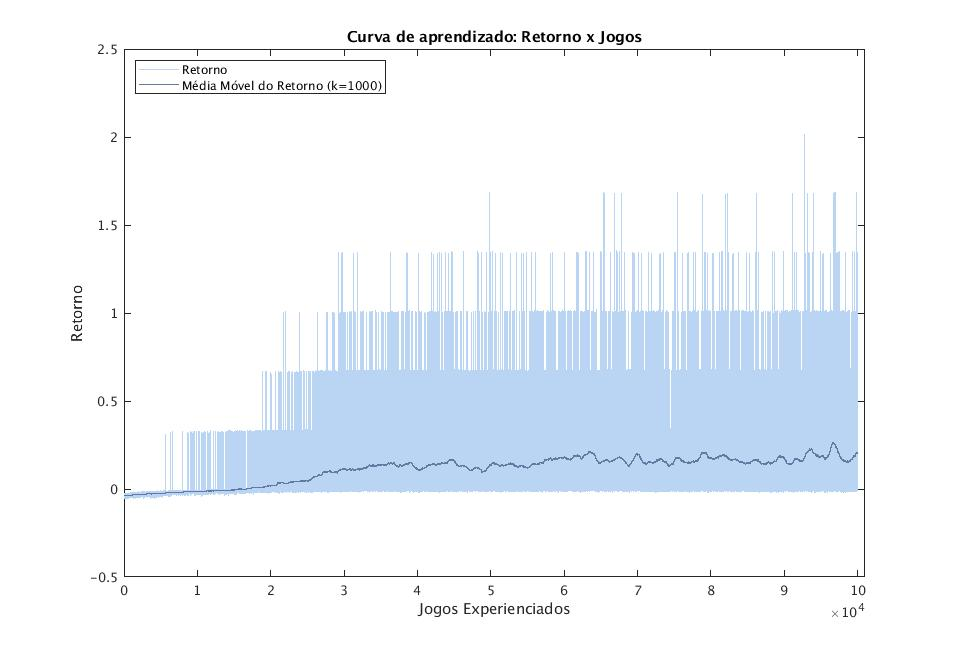
\includegraphics[width=1.0\linewidth]{figs/curva-qtabular.jpg}
	\centering
	\caption{Curva de aprendizado. Para cada jogo foi feita a média entre os 2 retornos observados em cada um dos treinamentos.}
	\label{fig:single-agent-curva}
\end{figure}

\section{Agentes Concorrentes}

Após validação do sistema com agente único, é interessante experimentar com treinamento adversarial de apenas 2 jogadores em formato um-contra-um. A intenção dessa etapa é experimentar com o sistema o caso adversarial, no qual há um ou mais agentes com objetivo oposto ao do agente sendo treinado.

\section{Múltiplos Agentes}

Após validar os casos de agente único e de agentes concorrentes, propõe-se um treinamento completo em jogos 11 contra 11. O objetivo é, ao final do processo, termos um time capaz de jogar contra os principais times da atualidade na categoria RoboCup Soccer Simulation 2D.

Para isso, os agentes devem ser capazes de cooperar e reagir aos movimentos da equipe oposta a fim de marcar gols e evitar os gols do adversário.


\begin{comment}
Resultados Experimentais
\end{comment}
\chapter{Resultados Experimentais}
\label{chap:Resultados}

% Gráficos e comentários provenientes de cada um dos experimentos.

% Resumo opcional. Comentar se não usar.
% \resumodocapitulo{Resumo opcional.}



\section{Sarsa Aproximado e Comportamentos Pré-Programados}

O treinamento utilizando o algoritmo Sarsa realizado contou com 30.000 partidas utilizando a rede neural multicamadas descrita na Subseção \ref{subsec:sarsadev} e salvando os retornos obtidos em cada partida.

O gráfico da Figura \ref{fig:single-agent-sarsa-behaviors} mostra em conjunto o retorno a cada partida e a média móvel do retorno com janela de 1000 partidas. É possível observar que há um tendência de subida do retorno com o passar dos episódios experienciados, porém em grande parte das partidas o agente não realizou nenhum gol, refletido pelo baixo valor da média de 100 partidas.

É interessante ressaltar o alto custo computacional deste tipo de treinamento devido à utilização de redes neurais. Dessa forma, a quantidade de amostras possíveis de serem coletadas em tempo hábil foram drasticamente reduzidas.

Além disso, a utilização de métodos aproximados posa um problema de duplo aprendizado: deseja-se aprender a política ótima enquanto se aprende a aproximar esta política ótima desconhecida por meio de uma rede neural. Esse fator contribui negativamente no tempo para convergência da política. Em métodos tabulares, apesar do maior custo de memória, esse problema é inexistente.

\begin{figure}[H]
	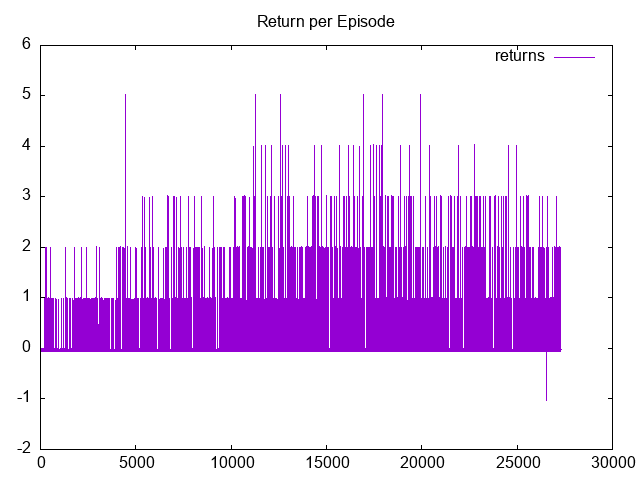
\includegraphics[width=0.9\linewidth]{figs/sarsa-tmp.png}
	\centering
	\caption{\textbf{[PLACEHOLDER]} Curva de aprendizado do agente com comportamentos pré-programados utilizando Sarsa aproximado.}
	\label{fig:single-agent-sarsa-behaviors}
\end{figure}

\section{\textit{Q-Learning} duplo Tabular e Comportamentos Pré-Programados}
\label{sec:behaviors-tabular}
Substituindo o aproximador de função por uma tabela e o algoritmo Sarsa pelo Q-Learning, foram executados 3 treinamentos de 100000 partidas e salvos a tabela Q completa e o histórico dos retornos obtidos pelo agente ao longo do treinamento.

O gráfico da Figura \ref{fig:single-agent-tabular-behaviors} mostra o histórico médio dos 3 treinamentos. Observa-se que
% o desempenho dessa abordagem supera o da abordagem anterior rapidamente, com poucas amostras. Em contrapartida, 
há uma estagnação do retorno por volta das 60000 amostras, o que pode indicar a necessidade de ajuste no decaimento do fator de exploração para que o agente explore novas possibilidades por mais partidas ou a existência de um limite superior para o desempenho do agente devido à menor flexibilidade da política aprendida, ou seja, o agente só é capaz de construir a política a partir dos comportamentos pré-programados.

\begin{figure}[H]
	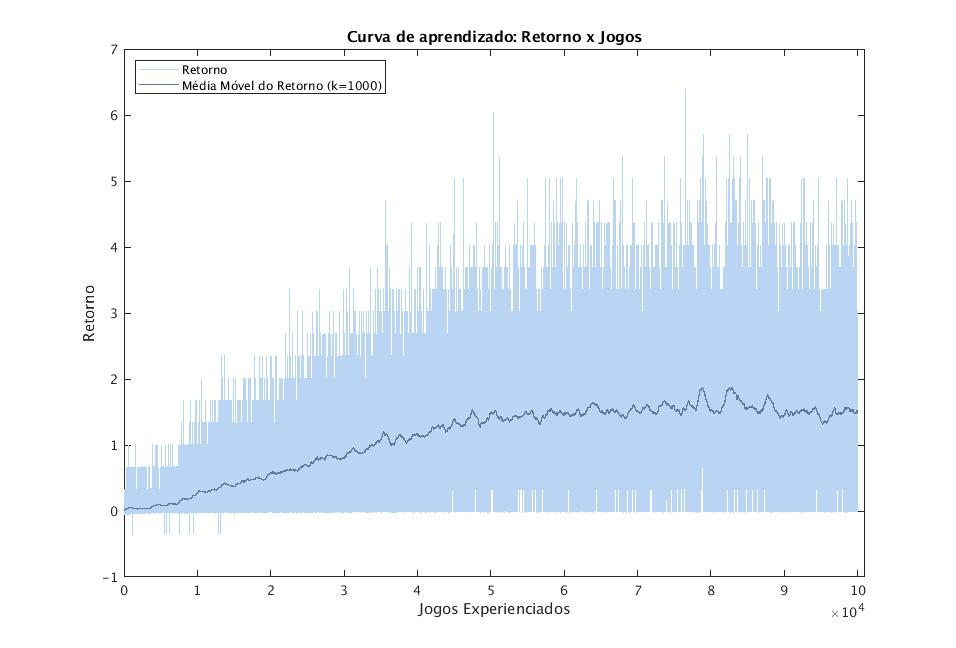
\includegraphics[width=0.9\linewidth]{figs/curva-behaviors-tabular.jpg}
	\centering
	\caption{Curva de aprendizado do agente com comportamentos pré-programados.}
	\label{fig:single-agent-tabular-behaviors}
\end{figure}

A Figura \ref{fig:goal-seq} ilustra o agente conduzindo a bola e realizando um gol conforme a política aprendida.

\begin{figure}[H]
	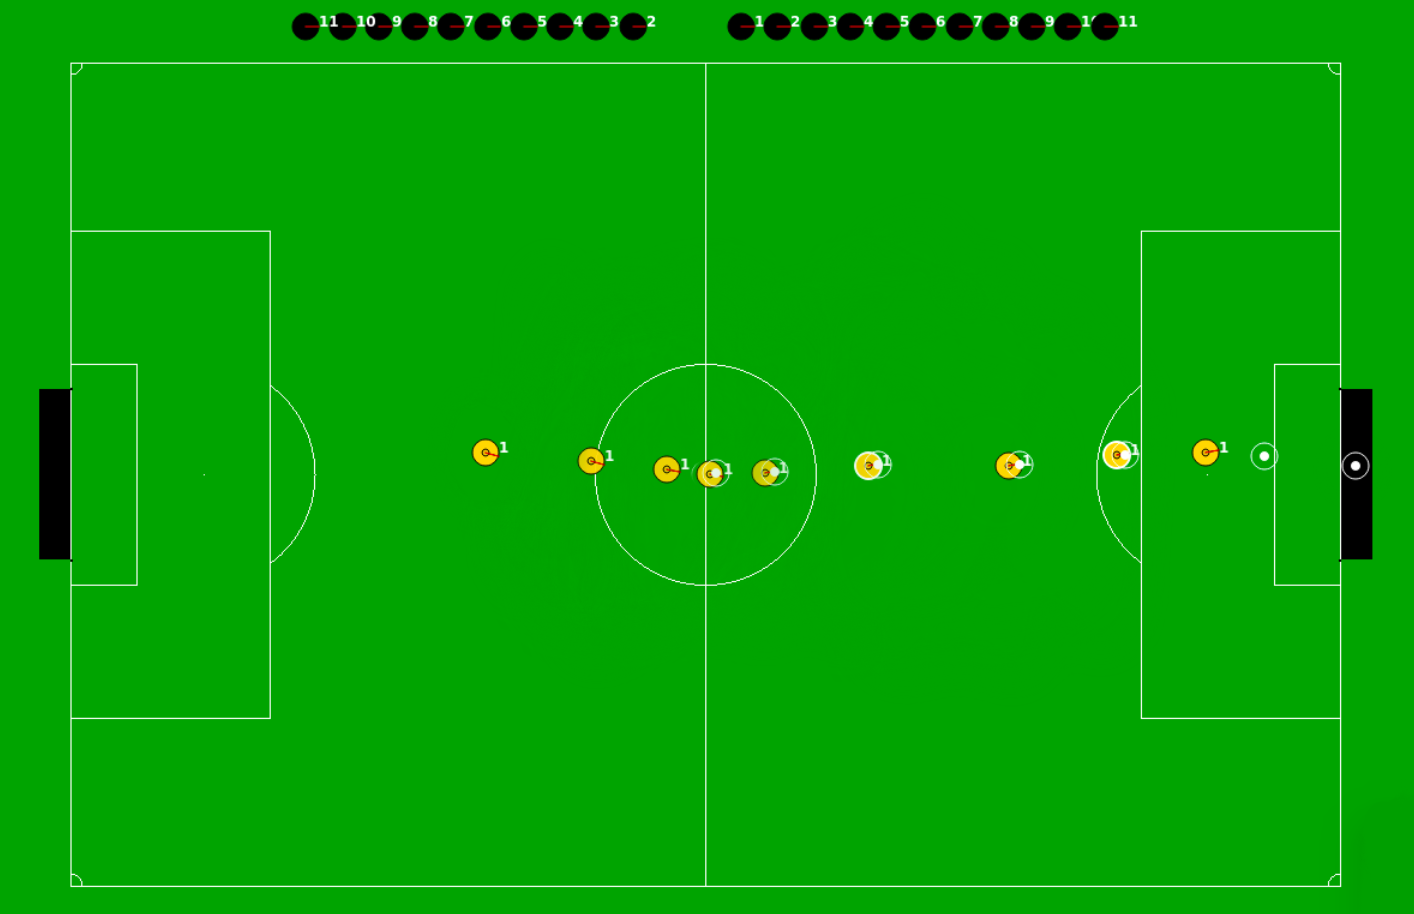
\includegraphics[width=0.9\linewidth]{figs/goal-sequence.png}
	\centering
	\caption{Sobreposição de sequência de imagens do agente fazendo gol.}
	\label{fig:goal-seq}
\end{figure}

A Figura \ref{fig:curvalonga-bhv} mostra o histórico de retornos para um treinamento mais longo, de 200000 partidas. Nela percebe-se que após a cessação da exploração o agente estabiliza seu desempenho um pouco abaixo do máximo obtido.

\begin{figure}[H]
	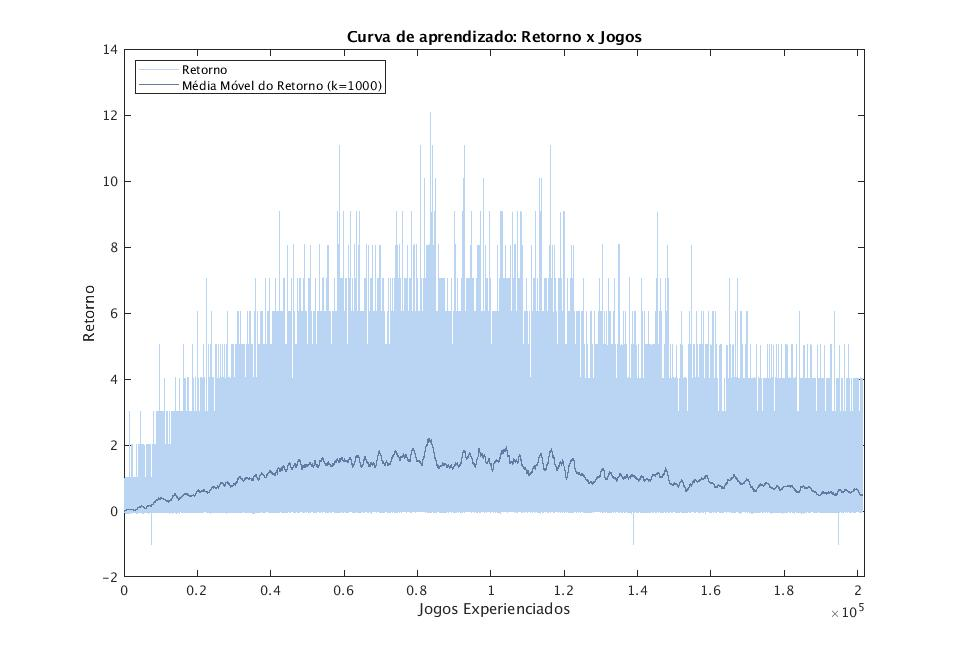
\includegraphics[width=0.9\linewidth]{figs/curvalonga-behaviors-tabular.jpg}
	\centering
	\caption{Curva de aprendizado do agente com comportamentos pré-programados para treinamento longo.}
	\label{fig:curvalonga-bhv}
\end{figure}

\section{\textit{Q-Learning} duplo Tabular e Ações Puras}

Substituindo os comportamentos pré-programados por uma seleção de ações puras, foram executados 3 treinamentos distintos de 100000 partidas a fim de suavizar o elemento sorte nos resultados. Após cada um dos treinamentos foram salvos a tabela Q completa e o histórico dos retornos obtidos pelo agente ao longo do treinamento.

A Figura \ref{fig:single-agent-curva} mostra esse histórico. É interessante observar que com o decaimento dos fatores de exploração e de aprendizagem, após 100000 partidas ambos eram $\epsilon \approx 0.074074$ e $\alpha \approx 0.056604$, ou seja, o agente já executava na maior parte dos ciclos a política aprendida. Para cada jogo foi feita a média entre os 3 retornos observados em cada um dos treinamentos.

\begin{figure}[H]
	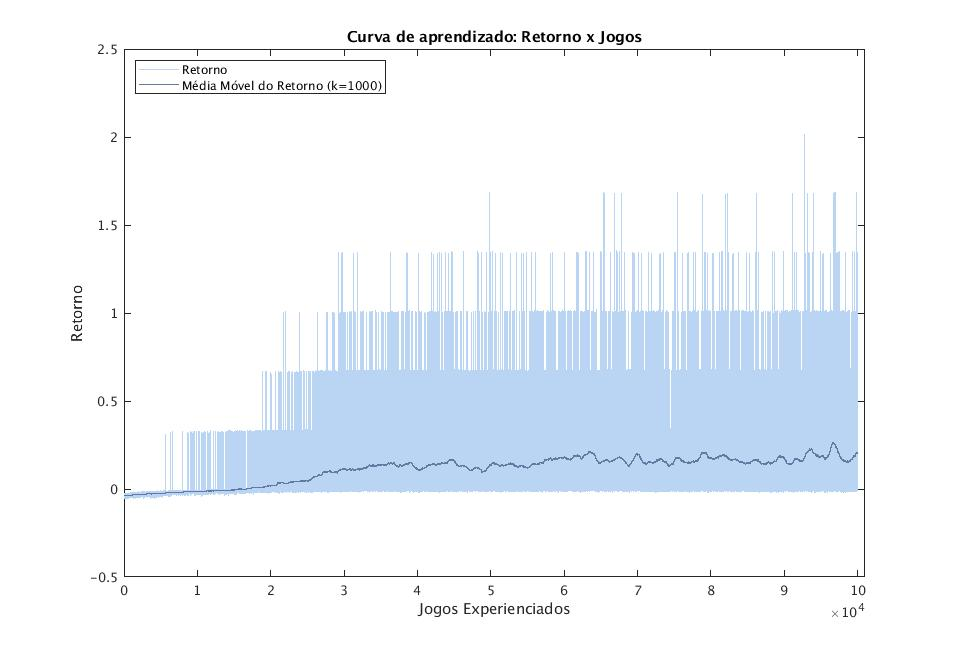
\includegraphics[width=0.93\linewidth]{figs/curva-qtabular.jpg}
	\centering
	\caption{Curva de aprendizado do agente com ações puras. }
	\label{fig:single-agent-curva}
\end{figure}

\begin{figure}[H]
	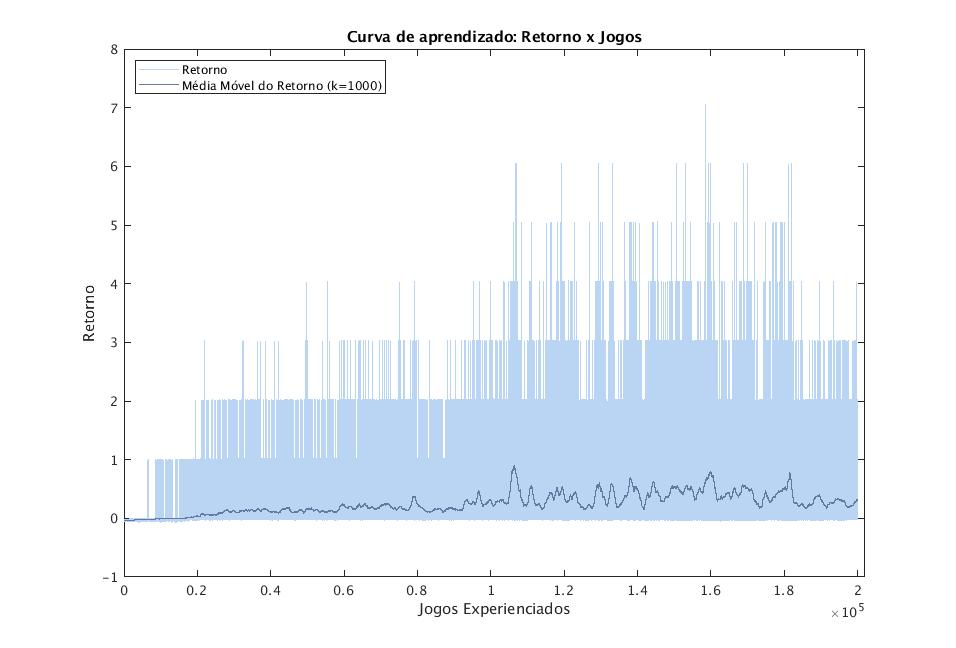
\includegraphics[width=0.93\linewidth]{figs/curvalonga-qtabular.jpg}
	\centering
	\caption{Curva de aprendizado para treinamento longo.}
	\label{fig:single-agent-curvalonga}
\end{figure}

Além disso, assim como na Seção \ref{sec:behaviors-tabular}, foi executado um treinamento de 200000 partidas a fim de observar a aprendizagem por um período mais longo. Na Figura \ref{fig:single-agent-curvalonga} observa-se que o agente continua melhorando seu desempenho até próximo do fim do treinamento, o que pode ser indício de que o aprendizado com ações puras de fato permite mais flexibilidade na política aprendida.

Apesar da grande quantidade de experiência a que o agente teve acesso, nota-se na Figura \ref{fig:single-agent-curvalonga} que o crescimento de seu desempenho é bastante limitado, sequer atingindo a média de 1 gol por partida. Isso é um indicativo do altíssimo custo computacional de soluções \textit{end-to-end} como a utilizada no experimento.

O capítulo seguinte relata as conclusões acerca desse trabalho, sua contribuição para a área e discorre sobre possíveis trabalhos para continuação do desenvolvimento da plataforma, especialmente dentro do contexto da Universidade de Brasília.

% \section{Agentes Concorrentes}

% Após validação do sistema com agente único, é interessante experimentar com treinamento adversarial de apenas 2 jogadores em formato um-contra-um. A intenção dessa etapa é experimentar com o sistema o caso adversarial, no qual há um ou mais agentes com objetivo oposto ao do agente sendo treinado.
 
% \section{Múltiplos Agentes}

% Após validar os casos de agente único e de agentes concorrentes, propõe-se um treinamento completo em jogos 11 contra 11. O objetivo é, ao final do processo, termos um time capaz de jogar contra os principais times da atualidade na categoria RoboCup Soccer Simulation 2D.

% Para isso, os agentes devem ser capazes de cooperar e reagir aos movimentos da equipe oposta a fim de marcar gols e evitar os gols do adversário.



\begin{comment}
Conclusões
\end{comment}

\chapter{Conclusões}
\label{chap:Conclusoes}
\par Este projeto teve como objetivo a implementação de uma plataforma para desenvolvimento de aprendizagem por reforço em futebol de robôs 2D e a utilização de técnicas de RL para realizar treinamentos de seleção de comportamentos e ações puras para maximizar o número de gols feitos por um agente.

\section{Plataforma para futebol de robôs}
\par Ao pesquisar sobre a comunidade e equipes participantes das edições nacionais da competição, notou-se que a biblioteca de interfaceamento com o servidor \textit{librcsc} e o time base \textit{agent2d} - ambos desenvolvidos no Japão por acadêmicos relacionados à equipe \textit{HELIOS} - são amplamente utilizados. Entretanto, a documentação da biblioteca é escassa e há dificuldade de utilização dela, evidenciado por conversas com os participantes da comunidade.
\par A plataforma desenvolvida no decorrer deste trabalho ajuda a modernizar e diversificar a base de código utilizada pelas equipes. A plataforma desenvolvida se encontra disponível em um repositório do GitHub: \textit{rcssggb/ggb-lib}, para ser utilizada livremente.

% \par Esse cenário demonstra a necessidade de modernização da base de código utilizada pelas equipes. É proposto, então, a reimplementação da interface de comunicação com o servidor da partida utilizando a linguagem Go.

% \section{Treinamento de Equipe para Participação em Competições}
% \par Este projeto propõe o treinamento de um time capaz de competir contra as principais equipes nacionais e internacionais da categoria. Serão estudados, avaliados e implementados métodos de inteligência computacional para o treinamento do time a fim de obter comportamentos adequados para os jogadores de modo que eles consigam atuar colaborativamente para vencer o time adversário.

% A participação em competições proporciona um ambiente perfeito para validação do sistema, uma vez que é possível comparar qualitativa e quantitativamente seu desempenho contra as diversas equipes do país.


\begin{comment}
Bibliografia
\end{comment}


\renewcommand{\bibname}{REFERÊNCIAS BIBLIOGRÁFICAS}
\addcontentsline{toc}{chapter}{REFERÊNCIAS BIBLIOGRÁFICAS}

\bibliographystyle{abnt-num}
\bibliography{bibliography}


\begin{comment}
Anexos
\end{comment}


% \anexos
\makeatletter
% não retirar estes comandos
\renewcommand{\@makechapterhead}[1]{%
  {\parindent \z@ \raggedleft \setfontarial\bfseries
\LARGE \thechapter. \space\space
\uppercase{#1}\par
\vskip 40\p@
}
}
\makeatother

\begin{comment}
Anexo I: Descrição do CD
\end{comment}


% 
\chapter{Descrição do conteúdo do CD}

\label{AnCD}

Descrever CD.


% \refstepcounter{noAnexo}

\begin{comment}
Anexo II: Programas Utilizados
\end{comment}


% 
\chapter{Programas utilizados}

Quais programas foram utilizados?


% \refstepcounter{noAnexo}

\begin{comment}
Acrescente mais anexos conforme julgar necessário.
\end{comment}

\end{document}
